\section{Deconvolution}
\subsection{Inverse filter}
The first and most obvious type of deconvolution is using an inverse filter. We have a blurred image $g$, we found an estimation of the psf ($h$) in the previous section. So we are theoretically ready to find the original image. We had
\begin{equation}
 g =  h*f,
\end{equation}
in frequency domain
\begin{equation}
G = HF. 
\end{equation}

Using $H$, the estimated psf in frequency domain, we can get $\hat{F}$ an so $\hat{f}$ by 
\begin{equation}
\hat{F} = H^{-1} G
\end{equation} 

However it's clear that if we add some noise this model doesn't work anymore. Indeed as shown on figure \ref{fig:psfFFT}, $H_e$ has some value near zero, especially at high frequencies because a blur typically reduces these frequencies. So when we divide $G$ by $H_e$, the noise is strongly amplified by the value near zero. This problem explains the results obtained on figure \ref{fig:inverseFilter}.   

\begin{figure}
\centering
%\missingfigure{T'as oublié de la pusher}
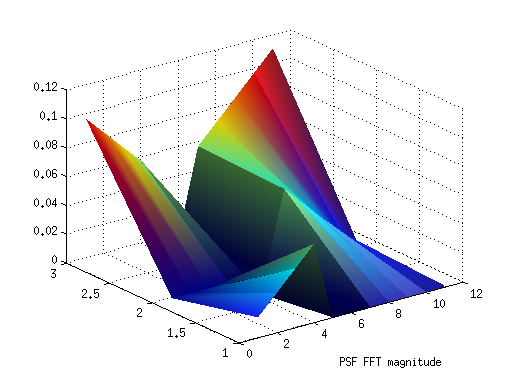
\includegraphics[scale=0.5]{../Images/psfFFT.png}
\caption{FFT of the psf}
\label{fig:psfFFT}
\end{figure}

\begin{myfig}{inverseFilter}
  {Effect of the noise with an inverse filter.}
  \mysubfig{matb-nonoise}{Image blurred without noise added}{0.32}
  \mysubfig{direct-nonoise}{Image deblurred without noise}{0.32}
  \mysubfig{matb-noisy}{Image blurred with noise added}{0.32}
  \mysubfig{direct-noisy}{Image deblurred with noise}{0.32}
\end{myfig}


\subsection{Lucy-Richarson}
\label{subsec:Lucy}
\subsubsection{Theory behind the method}
The method was introduced in~\cite{richardson1972bayesian} and
then in~\cite{lucy1974iterative} by Richarson and Lucy respectively.
I these articles, $f$ and $g$ are considered as probability function.
\cite{richardson1972bayesian} says (translated in our notations)
``Units of enery (which may be considered as unique events)
originating at a point in $f$ are distributed at points in $g$
according to the frequencies indicated by $h$''.
However, the justification of~\cite{richardson1972bayesian} (in 1D) uses
$P(f(x)) = \frac{f(x)}{\sum_x f(x)}$ which does not seem
very appropriate for our purpose.

When \cite{richardson1972bayesian} talks about energy,
that refers to the light which is quantized with photons.
That quantization gives us a reason to model the noise with
poisson distribution.
This modelization of the noise is called the shot noise and
is developped in~\cite{blanter2000shot}.
This model of the noise is used by~\cite{hebert1989generalized}.
\cite{temerinac2010tile} base on~\cite{hebert1989generalized}
and this model of the noise to show (even in 3D)
that the Lucy-Richardson algorithm gives the MLE of $f$ of this
model.

They suggest that $G \sim \pois(h * f)$ ($G$ is capitilize sinced it is a random function).
\todo{Show what we add to the proof and make it a theo}
Therefore,
\begin{align*}
  L(f) & = P(g|f)\\
  & = \prod_{(x,y)} \frac{[(h*f)(x,y)]^{g(x,y)} \exp(-(h*f)(x,y))}{(g(x,y))!}\\
  l(f) & = \sum_{(x,y)} g(x,y)\log((h*f)(x,y)) - (h*f)(x,y) -\log(g(x,y)!).
\end{align*}
Let's first develop
\begin{align*}
  \fpart{(h*g)(x,y)}{f(a,b)} & = \fpart{}{f(a,b)}\sum_{(i,j)}f(i,j)h(x-i,y-j)\\
  \fpart{(h*g)(x,y)}{f(a,b)} & = h(x-a,y-b).
\end{align*}
Consequently, we have
\begin{align*}
  \fpart{l(f)}{f(a,b)} & = \sum_{(x,y)} \left(\frac{g(x,y)}{(h*f)(x,y)} - 1\right) \fpart{(h*g)(x,y)}{f(a,b)}\\
  & = \sum_{(x,y)} \left(\frac{g(x,y)}{(h*f)(x,y)} - 1\right) h(x-a,y-b)\\
  & = \left(\left(\frac{g(x,y)}{(h*f)(x,y)} - 1\right) * h(-x,-y)\right)(a,b)\\
  & = \left(\left(\frac{g(x,y)}{(h*f)(x,y)}\right) * h(-x,-y)\right)(a,b) - 1 * h(-x,-y)\\
  & = \left(\left(\frac{g(x,y)}{(h*f)(x,y)}\right) * h(-x,-y)\right)(a,b) - \left(\sum_{(i,j)} h(-x-i,-y-j)\right)(a,b).
\end{align*}
As explained in the mathematical model,
\[ \sum_{(i,j)} h(i,j) = 1 \]
so we have
\[ \nabla l(f) = \frac{g(x,y)}{(h*f)(x,y)} * h(-x,-y) - 1. \]
To get the minimum of $l(f)$, $\nabla l(f)$ needs to be 0.
Therefore
\begin{equation}
  \label{eq:lucy-cond}
  \frac{g(x,y)}{(h*\hat{f})(x,y)} * h(-x,-y) = 1.
\end{equation}
If we multiply each side by $f(x,y)$, we get
\[ f(x,y)\left(\frac{g(x,y)}{(h*\hat{f})(x,y)} * h(-x,-y)\right) = f(x,y) \]
which can be solved iteratively using the fixed point method which gives us
\[ f_{k+1}(x,y) = f_k(x,y)\left(\frac{g(x,y)}{(h*f_k)(x,y)} * h(-x,-y)\right). \]

If we converge to $f$, we know that $\nabla l(f) = 0$
so $f$ is a critical point of $l(f)$.
However, we can't say that it maximize $l$ even
if we proof that the hessian is negatively definite since
the solution of the equation~\eqref{eq:lucy-cond}
is not unique.

For example, in 1-D, if
\begin{align*}
  h & = \frac{1}{2}
  \begin{pmatrix}
    1 & 1
  \end{pmatrix},\\
  g & =
  \begin{pmatrix}
    \cdots & 1 & 1 & 1 & \cdots
  \end{pmatrix},
\end{align*}
we have the two following solutions
\begin{align*}
  f_1 & = \frac{1}{2}
  \begin{pmatrix}
    \cdots & 1 & 1 & 1 & 1 & \cdots
  \end{pmatrix},\\
  f_2 & =
  \begin{pmatrix}
    \cdots & 0 & 2 & 0 & 2 & \cdots
  \end{pmatrix}.
\end{align*}
However, since $h * f_1 = h * f_2 = g$ so they maybe both maximize $l$.
%For example, in 1-D, if
%\begin{align*}
%  h & = \frac{1}{2}
%  \begin{pmatrix}
%    1 & 1
%  \end{pmatrix},\\
%  g & =
%  \begin{pmatrix}
%    \cdots & 1 & \frac{3}{2} & 1 & \frac{3}{2} & \cdots
%  \end{pmatrix},
%\end{align*}
%we have the two following solutions
%\begin{align*}
%  f_1 & = \frac{1}{2}
%  \begin{pmatrix}
%    \cdots & \frac{1}{2} & \frac{3}{2} & \frac{3}{2} & \frac{1}{2} & \frac{5}{2} & \cdots
%  \end{pmatrix},\\
%  f_2 & =
%  \begin{pmatrix}
%    \cdots & 3 & 1 & 2 & 2 & 1 & 3 & 1 & 2 & 2 & 1 & \cdots
%  \end{pmatrix}.
%\end{align*}

\subsubsection{Intuitive understanding}
\label{sec:lucy-intuitive}
A big advantage with this method is that we can understand
it intuitively.
Let's analyse an iteration.
\begin{enumerate}
  \item We start with an estimate $f_k$ and we compute
    $h * f_k$ which would be $g$ if $f_k = f$.
  \item We then compute, for each pixel, the ratio between
    the expected value $g(x,y)$ and what we currently have
    (i.e.  $(h * g)(x,y)$).
    Let's call it $r(x,y)$.
  \item If $h$ was $\delta(x,y)$, we could just take
    $f_{k+1} = f_k \cdot r$ and we would be done in one
    iteration.
    But here $g(x,y)$ is not only influenced by
    $f(x,y)$ but also by neighbouring values of $f$.
  \item The idea is therefore to spread $r$ on the values
    that have influenced $g(x,y)$.
    And $r(x,y)$ will influence a pixel in $f_k$ with the same
    weight that it influence $g(x,y)$.
    That's why we convolve $r$ with $h(-x,-y)$.
  \item Since each pixel has a sum of weight of 1,
    it will be influenced by a weight of 1 of elements of $r$.
    The ratio in $r(x,y) * h(-x, -y)$ is then multiplied to
    $f_k(x,y)$ to get $f_{k+1}(x,y)$.
\end{enumerate}
\[ f_{k+1}(x,y) = f_k(x,y)\left(\frac{g(x,y)}{(h*f_k)(x,y)} * h(-x,-y)\right). \]

\subsubsection{Practical case}
For the train case, $f$ and $g$ are given in a finite rectangle
and they have the same size which causes problems on their borders.
To compute $h * f$ on the border of $f$ we do not have enough
information. The same problem appears when we need to
convolve with $h(-x,-y)$.

Let's take an example with a 1-D blur to the right
2 pixels long. The first index is 1 and the last is $n$.
\begin{itemize}
  \item For the convolution with $h(-x,-y)$,
    we have a problem with $f(n)$ because it influences
    $g(n)$ and $g(n+1)$ and since $g(n+1)$ is unknown.
    A solution would be to only listen to the feedback given
    by $g(n)$ but the sum of the weight of the feedbacks
    will not be 1.
    Consequently, we need to modify the method.
    We will not spread $r$ but $r-1$ and then do $+1$
    after the convolution with $h(-x)$ which gives (in 2-D)
    \begin{equation}
      \label{eq:lucy_iter_modif}
      f_{k+1}(x,y) = f_k(x,y)\left(1+\left(\frac{g(x,y)}{(h*f_k)(x,y)}-1\right) * h(-x,-y)\right).
    \end{equation}
    That way, $f(n)$ is influenced by $g(n)$ the same
    way it influence $g(n)$ which seems mandatory and
    the effet of $g(n+1)$ is the same as if
    $g(n+1) = (h*f)(n+1)$.
  \item For $h * f$,
    let's assume that we have a 1-D blur to the right of 2 pixels
    (index starting at 1).
    $(h*f)(1)$ depends on both $f(1)$ and $f(0)$ but $f(0)$ is not processed.
    \begin{enumerate}
      \item An first idea would be to make $f$ starts at 2.
        We would approximate $\hat{f}(1)$ with $g(1)$.
        $g(2)$ will be influence by $f(2)$ which is being estimated
        and $\hat{f}(1)$ which is considered to be known.
        The only difference will be that we do not update $\hat{f}(1)$
        each iteration.
        To get an better estimate for $\hat{f}(1)$, we can take
        $g(1+L/2)$ where $L$ is the length of the blur since
        that is the mean of the $L/2$ neighbours on the right and left
        of $g(1)$.
        Let's call this method ``crop-lucy'' since it crops the image.
        We have implemented the first idea, which is to approximate
        $\hat{f}(1)$ with $g(1)$ since it was easier to implements
        and our faith was more in ``magic-lucy''.
      \item A second idea would be to estimate $f$ from 0
        which would only be influenced by $g(1)$.
        We would therefore use equation~\eqref{eq:lucy_iter_modif}
        for the iteration for the reasons explained earlier.
        For the general case, we add pior values of $f$ to the
        estimation process until $2-L$.
        With this method, we will estimate an image larger than
        the original image.
        We cannot hope to achieve it perfectly since the degrees since
        we have more unknowns than constraints but allowing
        lucy to search for values beyond the borders actually helps
        remove artifacts due to borders.
        Since estimating more pixels that we have on the blurred image
        is considered impossible and we are trying to do it,
        let's call this method ``magic-lucy''.
    \end{enumerate}
\end{itemize}

For $f_0$ we usually start with a gray image (unicolor) which gives acceptable results.
That way,
\begin{align*}
  f_1(x,y) & = f_0(x,y)\left(\frac{g(x,y)}{(h*f_0)(x,y)} * h(-x,-y)\right)\\
               & = F_0\left(\frac{g(x,y)}{F_0} * h(-x,-y)\right)\\
               & = g(x,y) * h(-x,-y).
\end{align*}
which is already correct if $g$ is unicolor.

\begin{myfig}{cameraman-magic}
  {Analysis of ``magic-lucy'' for the cameraman with 100 iterations.}
  \mysubfig{cameraman-g-60_30-black}{Cameraman blurred with zeros beyond the borders.}{0.32}
  \mysubfig{cameraman-fullmagic-60_30-black}{\figref{cameraman-g-60_30-black} deblurred ``magic-lucy''.}{0.32}
  \mysubfig{cameraman-f-60_30-black}{\figref{cameraman-g-60_30-black} deblurred by ``magic-lucy'' then cropped.}{0.32}
  \mysubfig{cameraman-g-60_30-circ}{Cameraman blurred with a circular image beyond the borders.}{0.32}
  \mysubfig{cameraman-fullmagic-60_30-circ}{\figref{cameraman-g-60_30-black} deblurred ``magic-lucy''.}{0.32}
  \mysubfig{cameraman-f-60_30-circ}{\figref{cameraman-g-60_30-black} deblurred by ``magic-lucy'' then cropped.}{0.32}
\end{myfig}

\begin{myfig}{cameraman-otherlucy}
  {Analysis of ``lucy'' and ``crop-lucy'' for the cameraman with 100 iterations.}
  \mysubfig{cameraman-lucy-60_30-black}{\figref{cameraman-g-60_30-black} deblurred by ``lucy''.}{0.45}
  \mysubfig{cameraman-lucy-60_30-circ}{\figref{cameraman-g-60_30-circ} deblurred by ``lucy''.}{0.45}
  \mysubfig{cameraman-croplucy-60_30-black}{\figref{cameraman-g-60_30-black} deblurred by ``crop-lucy''.}{0.45}
  \mysubfig{cameraman-croplucy-60_30-circ}{\figref{cameraman-g-60_30-circ} deblurred by ``crop-lucy''.}{0.45}
\end{myfig}

To illustrate this method, let's see what it does on the cameraman
with the \figref{cameraman-magic}.
We have blurred it with a black extrapolation beyond the borders
(see \figref{cameraman-g-60_30-black}) and with circular extrapolation
(see \figref{cameraman-g-60_30-circ}).

We can see that ``lucy'' has a lot of troubles with the black
extrapolation but not with the circular interpolation.
``lucy'' is done by the \lstinline|deconvlucy| function of MATLAB.
We can guess that at each iteration of lucy,
\lstinline|deconvlucy| do convolutions with ``replicate''
extrapolation beyond the borders (set it to the pixel at the border).
That's why it has trouble with the black extrapolation since this is
very different from the pixel at the border.
On the other hand, with the circular interpolation,
the extrapolation is quite similar to the pixel at the border due
to the borders of the cameraman being quite symmetrical.

``crop-lucy'' doesn't work well due to the approximation of the pixels
cropped which is not terrific.
It makes this error propagate to all the images through the iterations.

With those 2 examples, we can see the problems of many iterations.
If we have errors (like the borders here), the more iterations
we make, the more the error is propagated.

On the other hand, ``magic-lucy'' thrives.
We can see in~\figref{cameraman-fullmagic-60_30-black}
that the extrapolation used has been correctly estimated.
For \figref{cameraman-fullmagic-60_30-circ},
on the left, it is extraordinarily accurate we even have the white
spot at the limite between the ground and the sky present at the right of the image.
Since the blur is circular, it appears there, which was expected.
On the bottom, it has more trouble since the sky is quite different to the
ground and our problem is underdetermined.
Anyway, \figref{cameraman-f-60_30-circ} has no border artifacts which
is the purpose.

\subsection{Wiener}
\label{subsec:Wiener}
 Another deconvolution is the wiener one. The wiener filter is more robust than the inverse filter because it doesn't ignore the noise. We have in the frequency domain
\begin{equation}
G(k,l) = H(k,l)F(k,l) + N(k,l),
\label{eq:FeHF}
\end{equation} 
 where $N$ is the DF transform of a noise $n$ with mean $0$. We want to estimate $\hat{F}$ based on the image observed $F$ and a filter $L$ which still need to be defined, i.e. 
 \begin{equation}
\hat{F}(k,l) = L(k,l)F(k,l).
 \label{eq:feLF}
 \end{equation}

We want a filter $L$ such as it minimizes 
\begin{equation}
\min \mathbb{E}\{|F(k,l) - \hat{F}(k,l)|^2\},
\label{eq:FFe}
\end{equation}
and so, using equations \eqref{eq:FeHF} and \eqref{eq:feLF} we can transform equation \eqref{eq:FFe} (we don't write $(k,l)$) in 
\begin{align*}
\mathbb{E}\{|F - \hat{F}|^2\} &= \mathbb{E}\{|F - L(HF+N)|^2\}\\
	&= \mathbb{E}\{|(1-LH)F - LN|^2\}
\end{align*}

Then, let's introduce some notations concerning the power spectrum :
\begin{itemize}
\item $S_f(k,l) = \mathbb{E}\{|F(k,l)|^2\}$ is the signal power spectrum
\item $S_n(k,l) = \mathbb{E}\{|N(k,l)|^2\}$ is noise power spectrum 
\end{itemize}

After some computation and taking the derivative, we get

\begin{equation}
L(k,l)= \frac{H^*(k,l)+S_f(k,l)}{|H|^2 S_f(k,l) + S_n(k,l)}.
\label{eq:LsemiFinal}
\end{equation}

Finally, defining $NSR = \frac{S_n}{S_f}$, we can rewrite $L$ as 
\begin{equation}
L (k,l)= \frac{H^*(k,l)}{|H(k,l)|^2 + NSR}.
\end{equation}
and 
\begin{equation}
 \hat{F}(k,l) = \frac{H^*(k,l)}{|H(k,l)|^2 + NSR} G(k,l).
\end{equation}
So the filter $L$ gives the minimum mean-square error estimate of $F$.
However, this filter needs an estimation of the noise and image variances, which are difficult to estimate. For further details on this estimation, please refer to the section \ref{sec:NSREstimation}.

\subsection{Regularisation}
\label{subsec:Reg}
The last deconvolution method is the deconvolution using regularized filter. 
Instead of a simple inverse filter, we want to minimize the sum of two terms. The first one is the square of the error between the blurred image received and the blurred one using the psf and the original image we are looking for. The second term is used to smooth the image to a certain extent. 

\begin{equation}
\min \sum_{x,y} \left[ (g(x,y) - h(x,y)*f(x,y))^2 + \alpha (l(x,y)*f(x,y))^2 \right]
\end{equation}

And using the Fourier transform, we get
\begin{equation}
\min \sum_{k,l} \{ [G(k,l) - H(k,l)F(k,l)]^2 + \alpha [L(k,l)F(k,l)]^2\}
\label{eq:FTreg}
\end{equation}

The term $L(k,l)$ is chosen as a high pass filter in order to minimize the high-frequencies, i.e. the roughness in the solution. Indeed the noise is a high frequency in the frequency domain as it is a big change between two pixels. 

The parameter $\alpha$ controls the degree of roughness penalty. The higher the coefficient is, the smoother the image will be\cite{mathWorksWiener}. Indeed if $\alpha$ is big, it amplifies more the high frequencies from $LF$ and because we want to minimise the expression \eqref{eq:FTreg} the low frequencies will be preferred.

With the derivative we obtain
\begin{equation}
\hat{F}(k,l) = \frac{H(k,l)}{|H(k,l)|^2 + \alpha |L(k,l)|^2} G(k,l)
\end{equation}
So when the value of $H$ is near zero, the term $\alpha |L(k,l)|^2$ is there to avoid a too small denominator. 

